\chapter{Test of Vanna-Volga Pricing}


\section{Data Source}
\subsection{Volatility Matrix}
\paragraph{}
Volatity matrix data in terms of ATM, $10\Delta$, and 25$\Delta$ butterflies (BF) and risk reversals (RR) with three FX derivatives for Vanna-Volga models was sourced from Bloomberg. An example of volatility matrix data of EUR/USD observed on May 10, 2017 with 1M maturity was showing below.

\begin{figure}[htb]
	\centering
	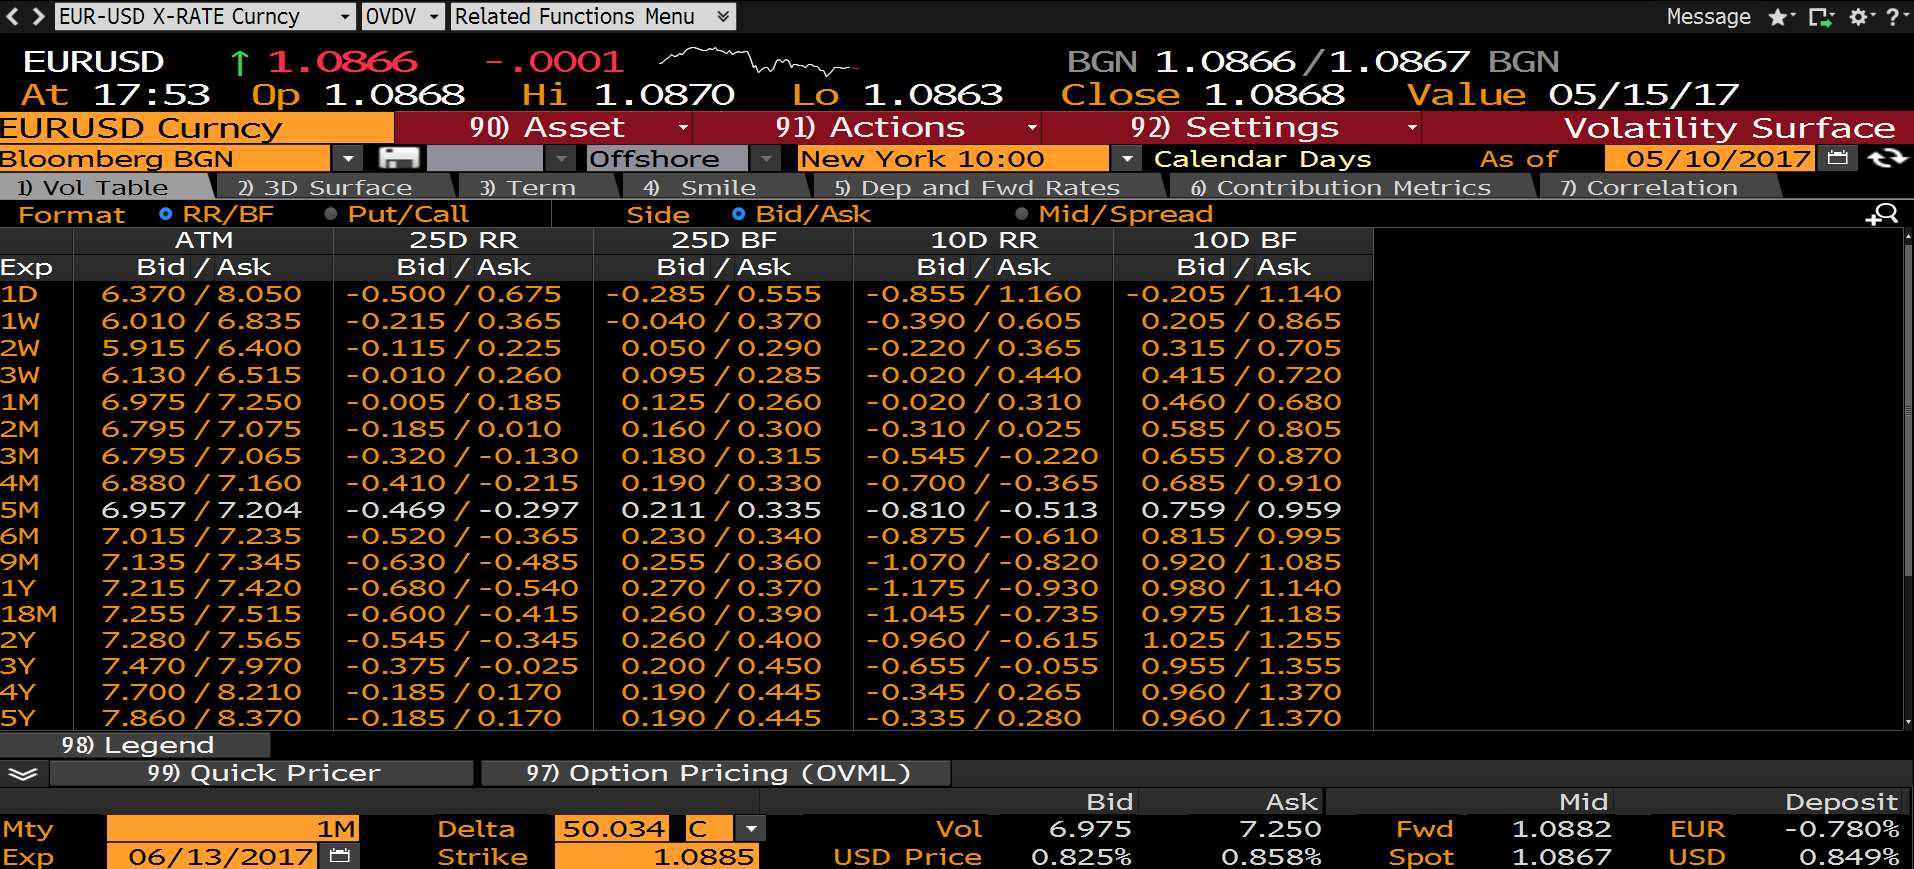
\includegraphics[scale=0.3]{./Testing-data/EURUSD.png} 
	\caption{Volatility matrix data in the bid/ask format in terms of ATM, $10\Delta$, and $25\Delta$ butterflies (BF) and risk reversals (RR), observed on May 10, 2017. Source: \textit{Bloomberg}}
	\label{fig:label} % insert suitable label, this is used to refer to a fig from within the text as shown above
\end{figure}
\paragraph{}
In order to verify the price calculated by using Vanna-Volga model, two benchmark sources (Bloomberg pricing model and \textit{investing.com} with price provided by \textit{Sentry Derivatives}) for all three FX derivatives had been put in \textit{Appendix 1}. Since Vanna-Volga is an analytically derived correction to Black-Scholes model, the price calucluated by Black-Scholes model also had been included for analysis.

\paragraph{}
The interest rates used for Vanna-Volga model and Black-Scholes model was obtained from \textit{www.tradingeconomics.com} and listed in the following table.

\begin{table}[htb]
\centering
\caption{{FX interest rates observed on May 10, 2017}}
\begin{tabular}{ccc}
\hline	\hline % insert double horizontal line
Symbol & USD & EUR   \\ [1ex]% heading
\hline
Rates & 1.00\% & 0.00\%    \\ [1ex]
\hline
\end{tabular}
\label{table:FX_rates}
\end{table}

\subsection{Model Implementation}
\paragraph{}
As the volatility matrix obtianed from Bloomberg is in the bid/ask format, the averaged mid volatility was used for Black-Scholes model and Vanna-Volga model. The mid volatility matrix data of three FX derivatives were list below. And we consider that live exchange rate as the initial price of FX options $S_0$.

\begin{table}[htb]
\centering
\caption{Mid volatiloty matrix}
\begin{tabular}{ccccccc}
\hline \hline
FX derivatives & ATM  & 25D RR  & 25D BF  & 10D RR  & 10D BF & $S_0$\\ [0.5ex]
\hline 
EUR/USD  & 7.1125 &0.09& 0.1925 &0.145 &0.57&1.0866 \\[0.5ex]
\hline
\end{tabular}
\end{table}

\paragraph{}
With the conventions and definitions specified in \textbf{Technical Specification}, the implementation of Black-Scholes model and Vanna-Volga model of FX derivatives had been coded in jupyter notebook with Python 3.5 in \textit{Appendix B}.

\section{Testing Results}
\paragraph{}

In order to compare the prices calculated from Vanna-Volga to the benchmark prices easily, we define the price to be \% FOR (foreign currency). For example, we use \% EUR to be the price form of Vanna-Volga model for EUR/USD options.

\paragraph{}
The results from the implemented codes with EUR/USD call option had been put in the following table. The details of the prices of four methods corresponding to the strike could be found in \textit{Appendix B}

\begin{table}[htb]
\centering
\caption{EUR/USD call option prices}
\begin{tabular}{ccccc}
\hline \hline
Strike & Bloomberg & investing.com & BS & Vanna-Volga \\ [0.5ex]
\hline
1.065 &	0.023241&	0.0233	&0.024682&	0.023363 \\ 
1.070&	0.019381&	0.0195&	0.020663&	0.019671\\
1.075	&0.015802&	0.0160&	0.016970&	0.016277 \\
1.080	&0.012571&	0.0128&	0.013649&	0.013224\\
1.085	&0.009770&	0.0101&	0.010733&	0.010544 \\ [0.5ex]
\hline
\end{tabular}
\label{table:prices}
\end{table}

\paragraph{}
From the table, we could find that the prices of Vanna-Volga were close to the prices of Bloomberg and investing.com. In particular, Vanna-Volga prices were very close to the prices used in investing.com. In order to visulize the results, a figure contained all the prices had been put in the below.

\begin{figure}[htb]
	\centering
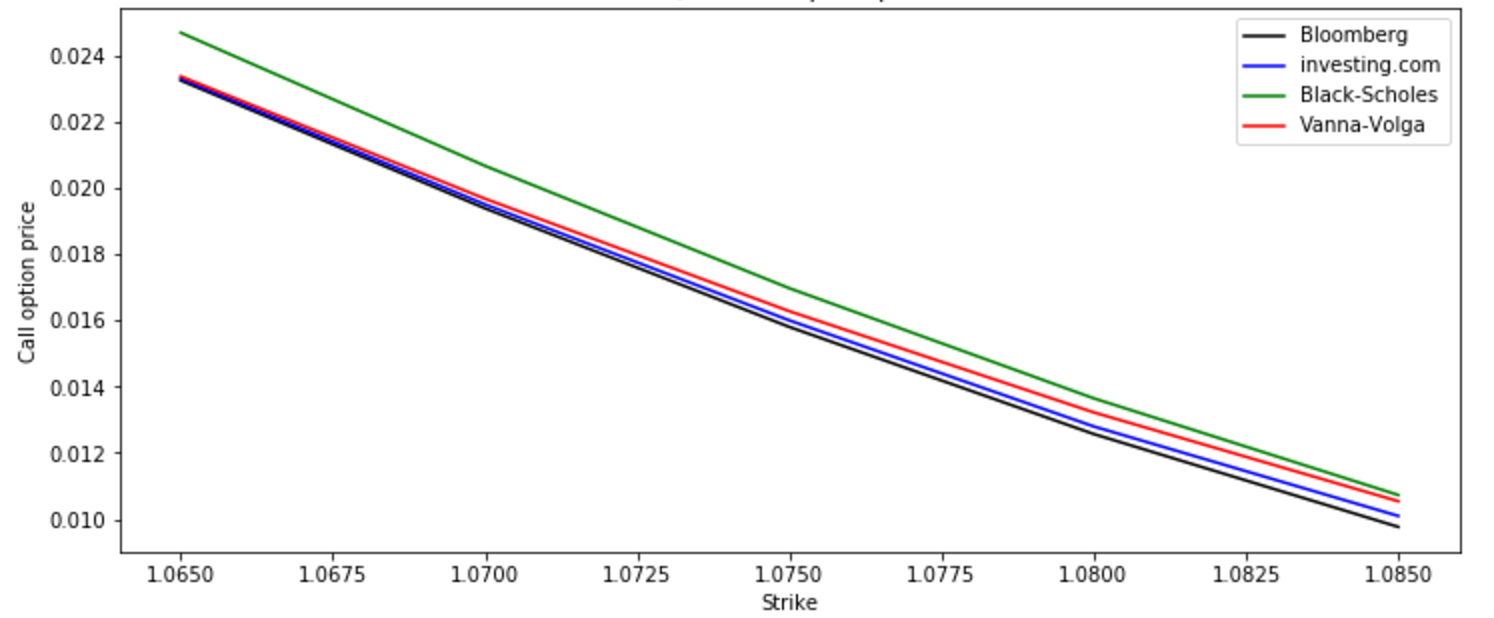
\includegraphics[scale=0.5]{./Testing-data/EURUSD-prices.png} 
\caption{Prices of EUR/USD call options with data observed on May 10, 2017}
\label{fig:prices-label} % insert suitable label, this is used to refer to a fig from within the text as shown above
\end{figure}

\paragraph{}
The figure clearly showed that the prices calculated through Vanna-Volga model were very close to the benchmark prices. Besides, as we might see, the Black-Scholes prices (green line) were far away from the benchmark prices compared to Vanna-Volga prices. This figure was consistent with the purpose of the Vanna-Volga model, which is that Vanna-Volga model is an analytically derived correction by capturing the greeks of vanna and volga to Black-Scholes model. Therefore, we consider the model is valid and approprite.